\chapter{Computational Homology}

Homology is one way of analyzing \textit{local} properties in order to extract information about \textit{global} phenomena. As large amounts of data become available, it becomes more difficult to determine what information is relevant. There are, of course, high and low-level approaches. A high-level approach like a fingerprint scanner or handwriting recognition might be the end-goal of one's analysis, but lower-level approaches like homology look at the geometric makeup of an object and is often a requisite step toward building higher-level processes.

	At this time, computational homology is a relatively new field and its application in physics has only recently been explored. Although homology is a field of algebraic topology, it combines the mathematics of several other fields including combinatorics and computation. The mathematical formalism behind homology is difficult to grasp so only the relevant information will be detailed in \refSect{ch2:imageanalysis}. \refSect{ch2:cubicalhomology} on cubical homology presents a more thorough discussion of the mathematical background of the topic while \JHedit{LATER SECTIONS to be written} provide an example of an algorithm to compute the homology.
	
\section{Image analysis} \label{ch2:imageanalysis}

To put it simply, homology is concerned with \textit{holes} and \textit{pieces}. Mathematically, how does one define a ``hole''? What does it mean to be part of a ``connected piece''? It's best to think about this in one dimension first. \refFig{fig:homology1d} shows two simple topological spaces, $X$ and $Y$. Although $X$ and $Y$ are spaces with one and two line segments respectively, in terms of homology one would say $X$ consists of a single \textit{connected piece} while $Y$ has two distinct pieces. The fact that the line segments are straight or of different length is not important for the homology. In this one-dimensional example, the \textit{zeroth homology groups} of each are

\begin{align}
	& H_0(X) \cong \mathbf{Z}^1  & \text{and} & \quad H_0(Y) \cong \mathbf{Z}^2
	\label{eq:homology1d}
\end{align}

where $\mathbf{Z}$ is the group of integers. The homology pairs a topological space (e.g.\ $X$ and $Y$) with an \textit{abelian group}, a set of elements combined with operations that satisfy five axioms (closure, associativity, identity, invertibility, and commutativity). Notice, however, that the \textit{zeroth homology group} of $Y$ is $\mathbf{Z}^2$; the rank of the group, $2$, is what accounts for the two ($2$) distinct pieces, but more on this later.

\begin{figure}
	\begin{center}
		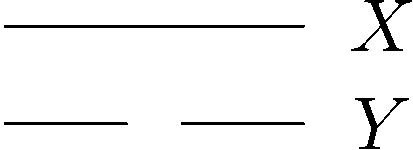
\includegraphics[width=0.2\columnwidth]{Figs/homology1d.pdf}
		\caption{\label{fig:homology1d} Topological spaces $X$ and $Y$. $X$ consists of one connected line segment and $Y$ has two disconnected line segments.}
	\end{center}
\end{figure}

Since there is a \textit{zeroth homology group}, it makes sense that there would be a \textit{first homology group}. Looking at the two-dimensional example in \refFig{fig:homology2d}, the homology of each space $X_a$, $X_b$, $X_c$, and $X_d$ is

\begin{align}
	H_1(X_a) \cong 0  & \quad H_1(X_b) \cong \mathbf{Z} & \quad H_1(X_c) \cong 0 & \quad H_1(X_d) \cong \mathbf{Z} \\
	H_0(X_i) \cong \mathbf{Z} & \qquad \text{for} & \quad i = a, b, c, d \label{eq:homology2d}
\end{align}

\begin{figure}
	\begin{center}
		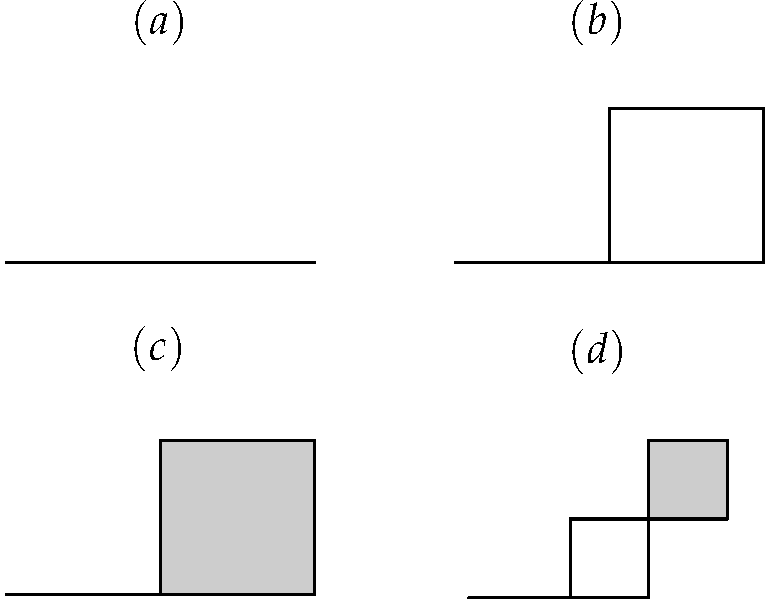
\includegraphics[width=0.6\columnwidth]{Figs/homology2d.pdf}
		\caption{\label{fig:homology2d} Topological spaces $X_a$, $X_b$, $X_c$, and $X_d$.}
	\end{center}
\end{figure}

All spaces $X_i$ for $i = a,b,c,d$ have a \textit{zeroth homology group} of $\mathbf{Z}$ since there is a single connected component. In \refFig{fig:homology2d}(b)-(c), the connected component forms an enclosed area (\eg the squares). The square in (b) forms a ``hole''. The shading indicates that the hole is filled and is thus no longer a ``hole''. \refFig{eq:homology2d}(b), (d) both contain one hole while (a), (c) contain zero holes. Just as the \textit{zeroth homology group} is concerned with connected segments, the \textit{first homology group} is concerned with ``holes''.

The terms ``piece'' and ``hole'' are informal. Formally, we could say that the $k^{th}$ homology group, $H_k(X)$, represents the group of $k$-dimensional \textit{holes} of $X$ where a 0-dimensional \textit{hole} is merely the gap between two components (\eg $Y$ in \reffig{fig:homology1d}). As I alluded to earlier, the the rank of the homology group (\eg the rank $2$ of $\mathbf{Z}^2$ in \refeq{eq:homology1d}) represents the number of $k$ dimensional holes. This is called the \textit{Betti number} $\beta_k$. Indeed, Betti numbers are non-zero for all $k < d$ where $d$ is the dimension of the topological space. The Betti numbers are the most important feature of the homology in this thesis since it nicely provides a mathematical quantity to an otherwise visual characteristic of a topological space. Later on I will describe how this information has been used to elucidate information about the dynamics of a system.

\section{Cubical Homology} \label{ch2:cubicalhomology}

In cubical homology, topological spaces are represented as a collection of cubes. This thesis is concerned with digital images as topological spaces. Digital images are quite literally a collection of two-dimensional cubes, \textit{pixels}, thus a homology that examines these objects is a natural environment for examining the output of a computer simulation. In this section I present a brief mathematical description of cubical homology which closely follows that of\rf{gameiro_2005} and\rf{kaczynski_2007}. We'll start by defining elementary cubes which make up the building blocks for the theory. It is important to keep in mind here that one of the fundamental ideas in homology theory is to connect topological objects (\eg connected pieces and holes) to algebraic objects.

\begin{defn}
	An \textit{elementary interval} is an interval $I \subset \R$ of the form
	\begin{align*}
		I = [ l, l+1 ] \quad \text{or} \quad I = [l,l]
	\end{align*}
	for some $l \in \R$. To simplify notation, say $$[l] = [l, l]$$ is an interval containing a single point, a \textit{degenerate} interval. Intervals of the form $[l, l+1]$ are called \textit{nondegenerate}.
\end{defn}

\begin{defn}
	An \textit{elementary cube} $Q$ is a finite product of elementary intervals, $$ Q = I_1 \times I_2 \times \ldots \times I_d \subset \R^d $$ where each $I_i$ is an elementary interval. We denote the set of all elementary cubes in $\R^d$ as $\Kd$. \\
	The set of all elementary cubes, $\K$,
	$$ \K := { \bigcup_{d=1}^{\infty} } \Kd . $$
\end{defn}

\begin{defn}
	Let $Q = I_1 \times I_2 \times \ldots \times I_d \subset \R^d$ be an elementary cube. The \textit{embedding number} of $Q$ is defined to be $d$ which we denote by $\emb{Q}$. Interval $I_i$ is the $i\ith$ \textit{component} of $Q$ and is written $\mathord{I_i(Q)}$. The \textit{dimension} of $Q$ is defined as the number of nondegenerate components in $Q$ and denoted $\dim{Q}$. We refer to an elementary cube $Q$ with $\dim{Q} = k$ as a \textit{k-cube} and denote
	$$ \K_k := \{ Q \in \K | \dim{Q} = k \},$$ and
	$$ \K_{k}^{d} := \K_k \cap \Kd. $$
\end{defn}
The relationship between the embedding number and dimension might be a little muddy since it seems that they would always be the same. Observe that for elementary cube {Q}, if $\emb{Q} = d$, then $Q \in \Kd$. The only general relation between the embedding number and dimension of $Q$ is that $$ 0 \leq \dim{Q} \leq \emb{Q} .$$ To illustrate this, imagine a Rubik's cube on a desk. The Rubik's cube itself has both emb, dim $= 3$ while any one square \textit{face} has $\text{emb} = 3$ but $\dim = 2$ (also see \refEx{ex:embvsdim}).

\begin{exmp} \label{ex:embvsdim}
	Given elementary cube $Q := [1,2] \times [1,2] \times [-1] \subset \R^3$, we have $I_1(Q) = [1,2]$, $I_2(Q) = [1,2]$, and $I_3(Q) = [-1] (degenerate)$. Therefore, $\emb{Q} = 3$ and $\dim{Q} = 2$.
\end{exmp}

\noindent \JHedit{some examples should be added here later}
%%%%% ADD SOME EXAMPLES HERE LATER %%%%%

Now we must define the class of topological spaces for which we define the homology.

\begin{defn}
	A set $X \subset \R^d$ is \textit{cubical} if $X$ can be written as a finite union of elementary cubes.
\end{defn}

Given cubical complex $X \subset \R^d$, we define
	$$ \K(X) := \{ Q \in \K \, | \, Q \subset X \} $$ and
	$$ \K_k (X) := \{ Q \in \K (X) \, | \, \dim{Q} = k \}. $$
We can write $\Kd (X)$ to remind us that $X \subset \R^d$ as well as $\Kd_k := \Kd(X) \cap K_k(X)$. For example, elements of $\K_0(X)$ are \textit{vertices} of $X$, elements of $\K_1(X)$ are \textit{edges} and so forth. Then $\K_k(X)$ are the \textit{k-cubes} of $X$.

As previously mentioned, our goal is to have a relationship between algebraic objects and topological spaces. The first step, then, is to associate some algebraic object with the elementary cubes we just defined.

\begin{defn}
	For each elementary \textit{k-cube} $Q \in \Kd_k$, we associate an algebraic object $\Qhat$ which we call an \textit{elementary k-chain} of $\R^d$ where $\Qhat : \Kd_k \rightarrow \Z$ is the function defined by
	$$\Qhat(P) =
		\begin{cases}
			1	& \text{if } P = Q, \\
			0	& \text{otherwise.}
		\end{cases}$$
	We also define $0 : \Kd_k \rightarrow \Z$ to be the zero function, \ie $\wh{0}(Q) = 0$ for all $Q \in \Kd_k$.
	The set of all \textit{elementary k-chains} of $\R^d$ is given by
	$$ \wh{\Kd_k} := \left\{ \Qhat \, | \, Q \in \Kd_k \right\} $$ and the set of all \textit{elementary chains} of $\R^d$ is given by
	$$ \wh{\Kd} := { \bigcup_{k=0}^{\infty} } \wh{\Kd_k} . $$
\end{defn}

For an elementary cube $Q$, we refer to $\Qhat$ as its \textit{dual elementary chain}. Conversely, given elementary chain $\Qhat$, we call $Q$ is its \textit{dual elementary cube}. What we want is that there is a one-to-one relationship between the elementary \textit{k-cubes} (topological objects) and \textit{elementary k-chains} (algebraic objects). In other words, the map of \textit{k-cubes} ($\Kd_k$) to \textit{k-chains} ($\wh{\Kd_k}$) is a \textit{bijection}. 

\begin{prop} \label{prop:bijection}
	The map $\phi : \Kd_k \rightarrow \wh{\Kd_k}$ given by $\phi(Q) = \Qhat$ is a bijection.
\end{prop}

\begin{proof}
	See\rf{kaczynski_2007}.
\end{proof}

Proposition~\ref{prop:bijection} allows us invoke the inverse of $\phi$ to go from an algebraic object, the elementary chain $\Qhat$, to a topological set, $Q$. The following definition uses the algebra we've built up to give the elementary \textit{k-chains} algebraic structure.

\begin{defn}
	The group $C_k^d$ of \textit{k-dimensional chains} (or \textit{k-chains}) of $\R^d$ is the free abelian group generated by the elementary chains of $\Kd_k$. Thus the elements of $C_k^d$ are functions $c : \Kd_k \rightarrow \Z$ such that $c(Q) = 0$ for all but a finite number of $Q \in \Kd_k$.
\end{defn}

\JHedit{I really want to make this section very readable with nice figures and stuff}. \refFig{fig:boundaries} illustrates how we can use information about the boundary to exact information about the $k$-cubes, but we are again using topological information (the existence of a boundary) to derive more topological information (the existence of loops). What we would really like to do is use algebra to get at this information, so we start by defining the algebraic boundary of a $k$-chain.

\begin{figure}[htbp]
\begin{center}
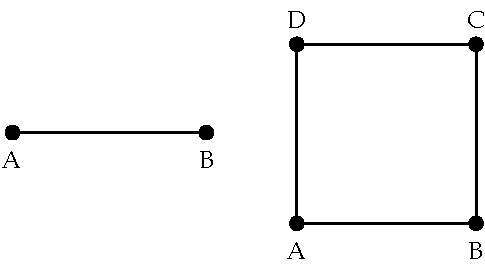
\includegraphics[width=0.5\columnwidth]{boundaries.pdf}
\caption{\label{fig:boundaries} The left picture has a boundary given by $\{ A \} \cup \{ B \}$ and therefore does not form a loop (a 0-cube). The picture on the right, however, does not have a boundary and therefore forms a loop (a 1-cube).}
\end{center}
\end{figure}











